
    \paragraph{Case where we have a 2-branch conditional}
    
    Figure~\ref{reord:cond_counter_example1(a)} shows an example of a program with conditionals (left) along with with its candidate execution (right) where the left conditional branch is taken and the outcome in the red box is not possible. 
    \begin{figure}[H]
        \centering 
        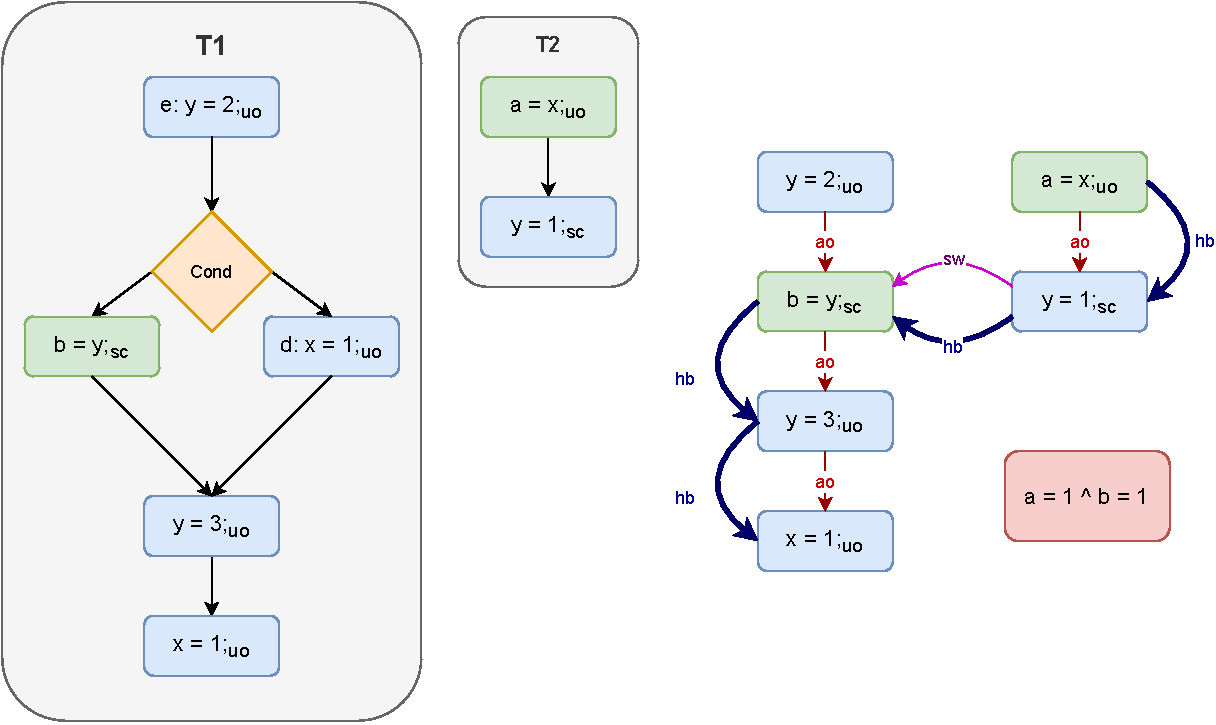
\includegraphics[scale=0.7]{7.CounterExamples/ReorderingConditionals/CounterExamples1a(Conditionals).pdf}
        \caption{Case with conditionals where $a = 1, b = 1$ is invalid due to Coherent Reads.}
        \label{reord:cond_counter_example1(a)}
    \end{figure}
    
    Observations:
    \begin{itemize}
        \item For $b=1$, it must come from the write $y=1_{sc}$. 
        Thus, we would have $\reln{\{y=1;_{sc}\}}{sw}{\{b=y;_{sc}\}}$ and hence $\reln{\{y=1;_{sc}\}}{hb}{\{b=y;_{sc}\}}$.
        \item Using this relation and $\stck{_{ao}}$, we can infer $\reln{\{a=x;_{uo}\}}{hb}{\{x=1;_{uo}\}}$.
        \item The above relation corresponds to Axiom \ref{CoRe}, from which we conclude that we cannot have $\reln{\{a=x;_{uo}\}}{rf}{\{x=1;_{uo}\}}$.
    \end{itemize}
    
    Figure~\ref{reord:cond_counter_example1(b)} shows the program after reordering (right) two writes in $T1$ along with its candidate execution (left) where the same left conditional branch is taken and the outcome in the orange box is possible. 
    \begin{figure}[H]
        \centering 
        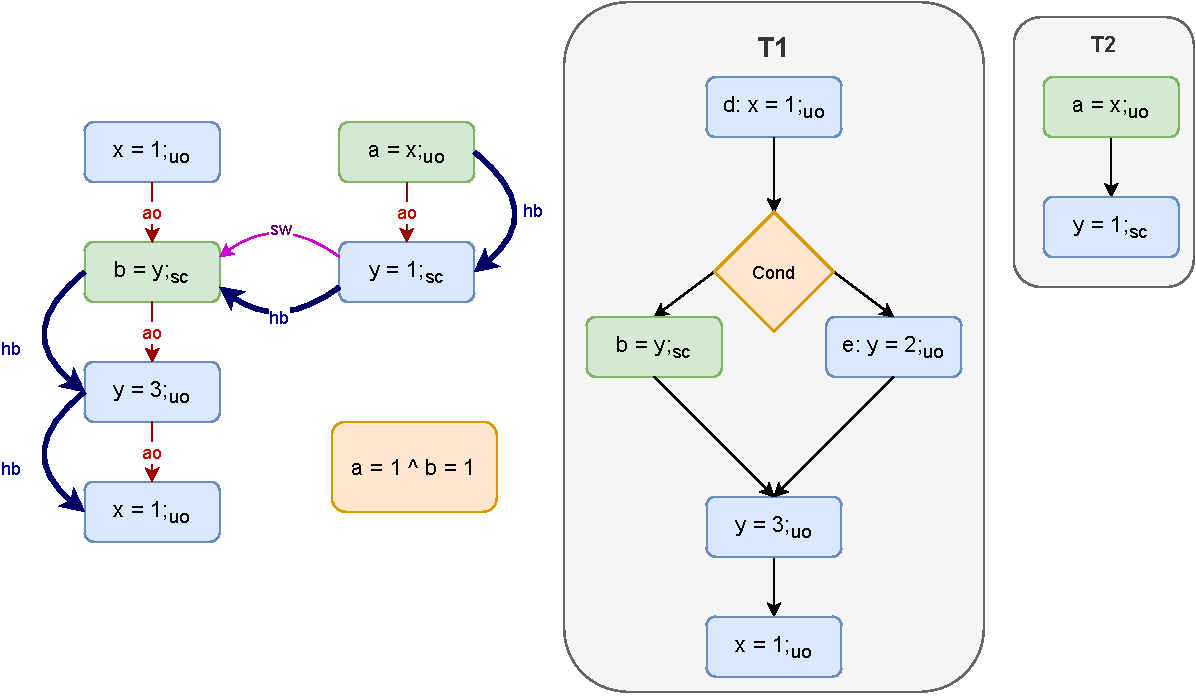
\includegraphics[scale=0.7]{7.CounterExamples/ReorderingConditionals/CounterExamples1b(Conditionals).pdf}
        \caption{Case where events of T1 are reordered, resulting in $a = 1,  b = 1$ to be valid.}
        \label{reord:cond_counter_example1(b)}
    \end{figure}
    
    Observations:
    \begin{itemize}
        \item For $b=1$, it must come from the write $y=1_{sc}$. 
        Thus, we would have $\reln{\{y=1;_{sc}\}}{sw}{\{b=y;_{sc}\}}$ and hence $\reln{\{y=1;_{sc}\}}{hb}{\{b=y;_{sc}\}}$.
        \item Now there is also event $d$, but there is no $\stck{_{hb}}$ relation between $d$ and $\{a=x_{uo}\}$.
        \item Thus for $a=1$, we can obtain this from event $d$. Thus, we can have the relation $\reln{\{a=x;_{uo}\}}{rf}{\{d: x=1;_{uo}\}}$.
    \end{itemize}
    
    \paragraph{Case with 1-branch conditional}

    Figure~\ref{reord:cond_counter_example2(a)} shows an example of a program (left) with 1-branch conditional along with with its candidate execution (right) where the conditional branch is not taken and the outcome in the red box is not possible. 
    \begin{figure}[H]
        \centering 
        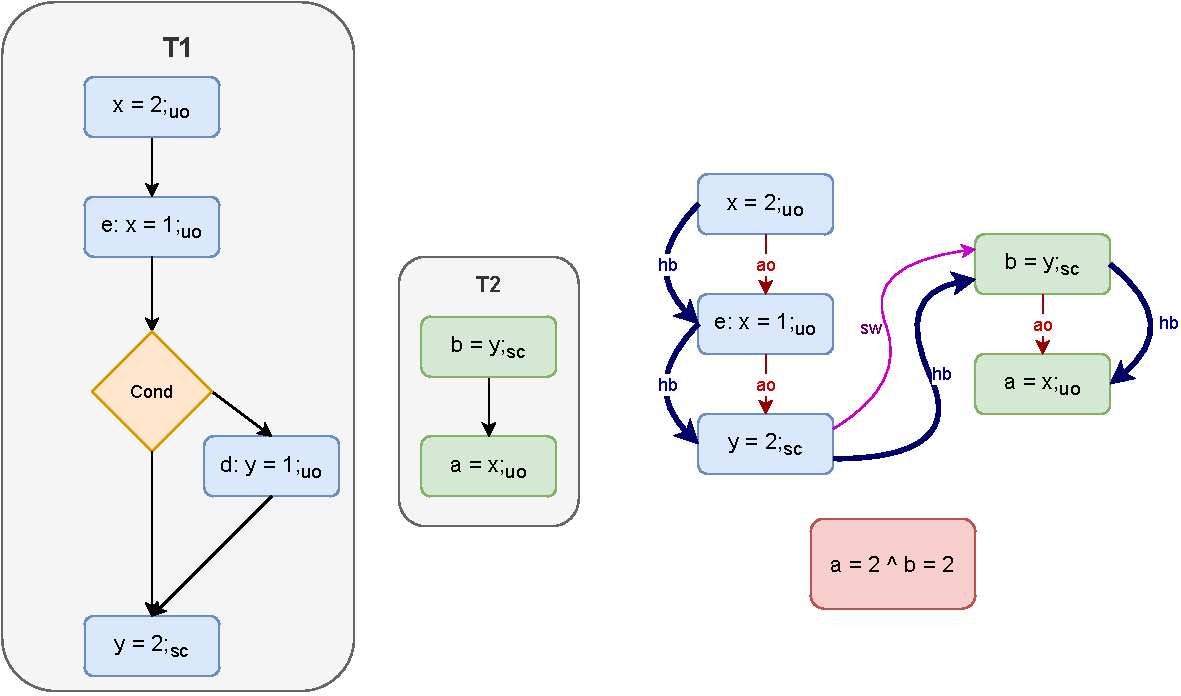
\includegraphics[scale=0.7]{7.CounterExamples/ReorderingConditionals/CounterExamples2a(Conditionals).pdf}
        \caption{Case with conditionals where $a = 2, b = 2$ is invalid due to Coherent Reads.}
        \label{reord:cond_counter_example2(a)}
    \end{figure}
    
    Observations:
    \begin{itemize}
        \item For $b=2$, it must come from the write $y=2_{sc}$. 
        Thus, we would have $\reln{\{y=2;_{sc}\}}{sw}{\{b=y;_{sc}\}}$ and hence $\reln{\{y=2;_{sc}\}}{hb}{\{b=y;_{sc}\}}$.
        \item From the above relation and $\stck{_{ao}}$, we can infer $\reln{\{x=2;_{uo}\}}{hb}{\reln{\{e: x=1;_{uo}\}}{hb}{\reln{\{y=2;_{sc}\}}{hb}{\reln{\{b=y;_{sc}\}}{hb}{\{a=x;_{uo}\}}}}}$.
        \item The above relation is a pattern of Axiom \ref{CoRe}, using which we can conclude that we cannot have $\reln{\{a=x;_{uo}\}}{rf}{\{x=2;_{uo}\}}$.
    \end{itemize}
    
    Figure~\ref{reord:cond_counter_example2(b)} shows the program after reordering (right) two writes in $T1$ along with its candidate execution (left) where the conditional branch is not taken and the outcome in the orange box is possible\footnotemark. 
    \begin{figure}[H]
        \centering 
        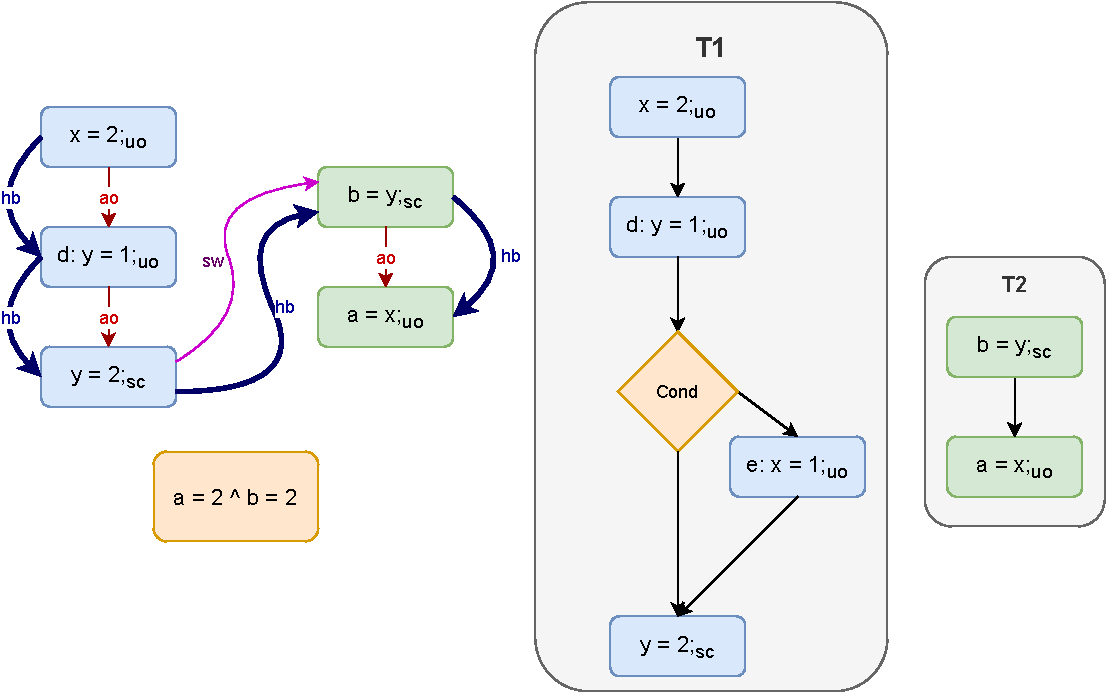
\includegraphics[scale=0.7]{7.CounterExamples/ReorderingConditionals/CounterExamples2b(Conditionals).pdf}
        \caption{Case where events of $T1$ are reordered, resulting in $a = 2,  b = 2$ to be valid.}
        \label{reord:cond_counter_example2(b)}
    \end{figure}

    \footnotetext{Notice that the above counterexample can also be attributed to the elimination of a write $x=1$.}
    Observations:
    \begin{itemize}
        \item For $b=2$, it must come from the write $y=2_{sc}$. 
        Thus, we would have $\reln{\{y=2;_{sc}\}}{sw}{\{b=y;_{sc}\}}$ and hence $\reln{\{y=2;_{sc}\}}{hb}{\{b=y;_{sc}\}}$.
        \item Because event $e$ is now within the conditional branch, we cannot have $\reln{\{e:x=1;_{uo}\}}{hb}{\{a=x;_{uo}\}}$.
        \item In addition, we have using the above inferred relation $\reln{\{x=2;_{uo}\}}{hb}{\{a=x;_{uo}\}}$.
        \item Hence, we can have the relation $\reln{\{a=x;_{uo}\}}{rf}{\{x=2;_{uo}\}}$.
    \end{itemize}
%-----------------------------------------------------------------------------------------------------------------------------------
    We leave the rest of the cases as an exercise to the avid reader\footnotemark.

    \footnotetext{While showing reordering of reads, one must note that the introduction of new observable behaviors is dependant on the fact that a candidate execution has a local variable reading a shared memory which must have not been there because a conditional branch was not taken. This fact, however, does not rely on the consistency rules of the memory model. Possible reason such a reordering helps could be that the compiler instantiates the local variables to some default value (say 0), and then decides to reorder a read outside a conditional on the assertion that the read will return the same constant value. Having such an assertion in general might not be always certain. This is one of the drawbacks of not using information as to why the compiler would do such a transformation.}
%------------------------------------------------------------------------------------------------------------------------------------------